% Options for packages loaded elsewhere
\PassOptionsToPackage{unicode}{hyperref}
\PassOptionsToPackage{hyphens}{url}
%
\documentclass[
]{article}
\usepackage{lmodern}
\usepackage{amssymb,amsmath}
\usepackage{ifxetex,ifluatex}
\ifnum 0\ifxetex 1\fi\ifluatex 1\fi=0 % if pdftex
  \usepackage[T1]{fontenc}
  \usepackage[utf8]{inputenc}
  \usepackage{textcomp} % provide euro and other symbols
\else % if luatex or xetex
  \usepackage{unicode-math}
  \defaultfontfeatures{Scale=MatchLowercase}
  \defaultfontfeatures[\rmfamily]{Ligatures=TeX,Scale=1}
\fi
% Use upquote if available, for straight quotes in verbatim environments
\IfFileExists{upquote.sty}{\usepackage{upquote}}{}
\IfFileExists{microtype.sty}{% use microtype if available
  \usepackage[]{microtype}
  \UseMicrotypeSet[protrusion]{basicmath} % disable protrusion for tt fonts
}{}
\makeatletter
\@ifundefined{KOMAClassName}{% if non-KOMA class
  \IfFileExists{parskip.sty}{%
    \usepackage{parskip}
  }{% else
    \setlength{\parindent}{0pt}
    \setlength{\parskip}{6pt plus 2pt minus 1pt}}
}{% if KOMA class
  \KOMAoptions{parskip=half}}
\makeatother
\usepackage{xcolor}
\IfFileExists{xurl.sty}{\usepackage{xurl}}{} % add URL line breaks if available
\IfFileExists{bookmark.sty}{\usepackage{bookmark}}{\usepackage{hyperref}}
\hypersetup{
  pdftitle={BDA Project: Hurricane forecasting in Stan},
  pdfauthor={José Miguel Ramírez \& Jonas Lindblad},
  hidelinks,
  pdfcreator={LaTeX via pandoc}}
\urlstyle{same} % disable monospaced font for URLs
\usepackage[margin=1in]{geometry}
\usepackage{color}
\usepackage{fancyvrb}
\newcommand{\VerbBar}{|}
\newcommand{\VERB}{\Verb[commandchars=\\\{\}]}
\DefineVerbatimEnvironment{Highlighting}{Verbatim}{commandchars=\\\{\}}
% Add ',fontsize=\small' for more characters per line
\usepackage{framed}
\definecolor{shadecolor}{RGB}{248,248,248}
\newenvironment{Shaded}{\begin{snugshade}}{\end{snugshade}}
\newcommand{\AlertTok}[1]{\textcolor[rgb]{0.94,0.16,0.16}{#1}}
\newcommand{\AnnotationTok}[1]{\textcolor[rgb]{0.56,0.35,0.01}{\textbf{\textit{#1}}}}
\newcommand{\AttributeTok}[1]{\textcolor[rgb]{0.77,0.63,0.00}{#1}}
\newcommand{\BaseNTok}[1]{\textcolor[rgb]{0.00,0.00,0.81}{#1}}
\newcommand{\BuiltInTok}[1]{#1}
\newcommand{\CharTok}[1]{\textcolor[rgb]{0.31,0.60,0.02}{#1}}
\newcommand{\CommentTok}[1]{\textcolor[rgb]{0.56,0.35,0.01}{\textit{#1}}}
\newcommand{\CommentVarTok}[1]{\textcolor[rgb]{0.56,0.35,0.01}{\textbf{\textit{#1}}}}
\newcommand{\ConstantTok}[1]{\textcolor[rgb]{0.00,0.00,0.00}{#1}}
\newcommand{\ControlFlowTok}[1]{\textcolor[rgb]{0.13,0.29,0.53}{\textbf{#1}}}
\newcommand{\DataTypeTok}[1]{\textcolor[rgb]{0.13,0.29,0.53}{#1}}
\newcommand{\DecValTok}[1]{\textcolor[rgb]{0.00,0.00,0.81}{#1}}
\newcommand{\DocumentationTok}[1]{\textcolor[rgb]{0.56,0.35,0.01}{\textbf{\textit{#1}}}}
\newcommand{\ErrorTok}[1]{\textcolor[rgb]{0.64,0.00,0.00}{\textbf{#1}}}
\newcommand{\ExtensionTok}[1]{#1}
\newcommand{\FloatTok}[1]{\textcolor[rgb]{0.00,0.00,0.81}{#1}}
\newcommand{\FunctionTok}[1]{\textcolor[rgb]{0.00,0.00,0.00}{#1}}
\newcommand{\ImportTok}[1]{#1}
\newcommand{\InformationTok}[1]{\textcolor[rgb]{0.56,0.35,0.01}{\textbf{\textit{#1}}}}
\newcommand{\KeywordTok}[1]{\textcolor[rgb]{0.13,0.29,0.53}{\textbf{#1}}}
\newcommand{\NormalTok}[1]{#1}
\newcommand{\OperatorTok}[1]{\textcolor[rgb]{0.81,0.36,0.00}{\textbf{#1}}}
\newcommand{\OtherTok}[1]{\textcolor[rgb]{0.56,0.35,0.01}{#1}}
\newcommand{\PreprocessorTok}[1]{\textcolor[rgb]{0.56,0.35,0.01}{\textit{#1}}}
\newcommand{\RegionMarkerTok}[1]{#1}
\newcommand{\SpecialCharTok}[1]{\textcolor[rgb]{0.00,0.00,0.00}{#1}}
\newcommand{\SpecialStringTok}[1]{\textcolor[rgb]{0.31,0.60,0.02}{#1}}
\newcommand{\StringTok}[1]{\textcolor[rgb]{0.31,0.60,0.02}{#1}}
\newcommand{\VariableTok}[1]{\textcolor[rgb]{0.00,0.00,0.00}{#1}}
\newcommand{\VerbatimStringTok}[1]{\textcolor[rgb]{0.31,0.60,0.02}{#1}}
\newcommand{\WarningTok}[1]{\textcolor[rgb]{0.56,0.35,0.01}{\textbf{\textit{#1}}}}
\usepackage{longtable,booktabs}
% Correct order of tables after \paragraph or \subparagraph
\usepackage{etoolbox}
\makeatletter
\patchcmd\longtable{\par}{\if@noskipsec\mbox{}\fi\par}{}{}
\makeatother
% Allow footnotes in longtable head/foot
\IfFileExists{footnotehyper.sty}{\usepackage{footnotehyper}}{\usepackage{footnote}}
\makesavenoteenv{longtable}
\usepackage{graphicx,grffile}
\makeatletter
\def\maxwidth{\ifdim\Gin@nat@width>\linewidth\linewidth\else\Gin@nat@width\fi}
\def\maxheight{\ifdim\Gin@nat@height>\textheight\textheight\else\Gin@nat@height\fi}
\makeatother
% Scale images if necessary, so that they will not overflow the page
% margins by default, and it is still possible to overwrite the defaults
% using explicit options in \includegraphics[width, height, ...]{}
\setkeys{Gin}{width=\maxwidth,height=\maxheight,keepaspectratio}
% Set default figure placement to htbp
\makeatletter
\def\fps@figure{htbp}
\makeatother
\setlength{\emergencystretch}{3em} % prevent overfull lines
\providecommand{\tightlist}{%
  \setlength{\itemsep}{0pt}\setlength{\parskip}{0pt}}
\setcounter{secnumdepth}{-\maxdimen} % remove section numbering
\usepackage{flafter}

\title{BDA Project: Hurricane forecasting in Stan}
\author{José Miguel Ramírez \& Jonas Lindblad}
\date{}

\begin{document}
\maketitle

{
\setcounter{tocdepth}{1}
\tableofcontents
}
\hypertarget{introduction}{%
\section{Introduction}\label{introduction}}

Tropical cyclones (in the Atlantic known as \emph{hurricanes}) are
destructive storms that occur during the late summer and fall in the
northern hemisphere's tropical region. The storms are usually classified
by their wind intensity in the region known as the \emph{eye wall},
i.e.~the circular region around the storm center where the wind speeds
are strongest. Highly intense hurricanes can cause extreme levels of
flooding in coastal areas and destroy buildings and homes. Furthermore,
the monetary damages and loss of lives seem to increase with an almost
exponential character as a function of storm intensity. As such, good
probabilistic forecasts of hurricane intensity are important for
purposes of evacuating areas at risk, as well as an interesting
scientific problem.

Meteorologists forecast hurricane intensity changes with two classes of
models: \emph{dynamical} models, or \emph{statistical} models. The
dynamical models are based on systems of differential equations that are
solved numerically with supercomputer clusters, while the statistical
models are based on black-box machine learning methods or more basic
statistical models. Rather bafflingly, one of the most successful models
is a multiple linear regression model called Statistical Hurricane
Intensity Prediction Scheme (SHIPS). Information about the SHIPS model
and its datasets are available at the website:
\href{http://rammb.cira.colostate.edu/research/tropical_cyclones/ships/index.asp}{SHIPS
Development}.

The reason that a model as simple as SHIPS is still in operational use,
is because of ongoing scientific challenges in understanding the complex
causes of (as well as impediments to) intensification. It is well-known
in the field that high sea temperatures in the tropical regions lead to
dissipation and convection, which intensifies hurricane winds, while
strong wind shear and surface drag causes weakening of the storms.
However, knowledge of these factors have not lead to a complete solution
to the problem and to some extent the issues may stem from the inherent
complexity and uncertainty in current remote sensing technology.

In this project, we develop models inspired by the SHIPS scheme and
using the SHIPS developmental data. The idea is to develop a Bayesian,
probabilistic, intensity forecast that could (in principle) be put into
operational use as a competitor to currently active statistical
hurricane models. Not being affiliated with a forecasting agency has its
limits however, as it is important to note that the SHIPS model also
uses information from the numerical weather forecasts run by the US
government. We do not have access to the global forecast models, and as
such are limited to creating a \emph{synoptic} model, i.e.~an intensity
forecast based purely on information available at the current time and
not using data from supercomputers that simulate the laws of physics.

\hypertarget{data}{%
\subsection{Data}\label{data}}

This project uses the `Developmental Data' from the SHIPS website:
\href{http://rammb.cira.colostate.edu/research/tropical_cyclones/ships/developmental_data.asp}{SHIPS
Developmental Data}. To be precise, we limit ourselves to the Atlantic
version of the SHIPS data, and use the data from the 5-day SHIPS
predictor file for the Atlantic. This data contains \textasciitilde140
variables in 6-hourly time steps for every hurricane season 1982-2019.
However, in this report we restrict the dataset to 2017-2019 in order to
make computation more tractable.

\hypertarget{description-of-the-variables}{%
\subsubsection{Description of the
variables}\label{description-of-the-variables}}

Describing all of the variables in the dataset is far outside the scope
of this document, although a few important quantities should be known to
the reader. Moreover, most of the variables are quite basic statistics
computed by taking averages over certain regions (usually a circle or
ring centered around the eye of the storm). The raw data used to compute
the variables is a global grid discretization of the atmosphere, while
the gridded discretization is created by statistically interpolating
data from satellite remote sensing, weather balloons, weather stations,
commercial/military aircraft, as well as weather buoys in the sea.

\textbf{Include a picture example to go along with how the variables are
computed?}

\textbf{Maximum wind speed (VMAX):} This is the current maximum wind
speed (in knots) in the eye wall of the hurricane, at \textasciitilde100
meters above surface. Actually, there may be gusts and turbulences that
are short-lived winds surpassing this wind speed, but it has been found
that the maximum \textasciitilde10 minute sustained winds in the eye
wall is simpler to measure and predicts maximum gusts and storm damages
best. In the Atlantic region this variable is measured by US military
aircraft that drop sondes inside the eye wall of the storm. In case
there is no scheduled flight mission to a hurricane, the maximum wind
speed is instead inferred using statistics and satellite observations.
Naturally, this is an estimate in either case, but the standard error is
in fact significantly lower when dropsonde measurements are used. In all
official US government data this quantity is rounded to the nearest
multiple of five (this includes the SHIPS dataset). The DELTA12 variable
corresponds to the value we want to predict: how the maximum wind speed
will change in 12 hours.

\textbf{Wind shear (SHRD):} Wind shear is the phenomenon where the wind
direction and speed differs significantly depending on height. The SHIPS
dataset contains several wind shear variables, since wind shear is known
to be an important variable that can impact the development of a
tropical storm. In regions with high wind shear, it can be very
difficult for a storm to intensify since excess energy is required for
the storm to maintain stability. Sometimes high wind shear can displace
and `rip apart' a storm, causing it to weaken and potentially dissipate.
Wind shear quantities are averages computed from wind data in the grid
discretization of the atmosphere.

\textbf{Sea temperature (CSST):} The main energy source for tropical
storms is the thermal energy in the sea, both the sea surface
temperature and the deeper ocean heat content. The SHIPS dataset
contains several variables representing the sea temperature, and these
are well-known to correspond to storm intensification. The main physical
process is that hot water evaporates, causing upward winds (convection)
that lower the pressure inside the eye of the storm. This in turn causes
winds to intensify as larger masses of the atmosphere get pushed towards
the low-pressure point in the storm eye. These quantities are based on
direct measurements from buoys and satellite remote sensing.

We will also be studying the effect of different subsets of the full
SHIPS set of variables. The first data set will only contain the wind
shear (SHRD) and the sea temperature (CSST), we will call from now on to
this dataset as ``B''. We will also study a dataset containing the same
variables as in ``A'' plus an extra variable: the maximum potential
intensity (VMPI), we will be refering to this dataset as ``B''. Finally,
we will also test a larger dataset with the variables SHRD, CSST, VMPI,
RHLO, and T200, we will refer to this dataset as ``C''.

\begin{figure}
\centering
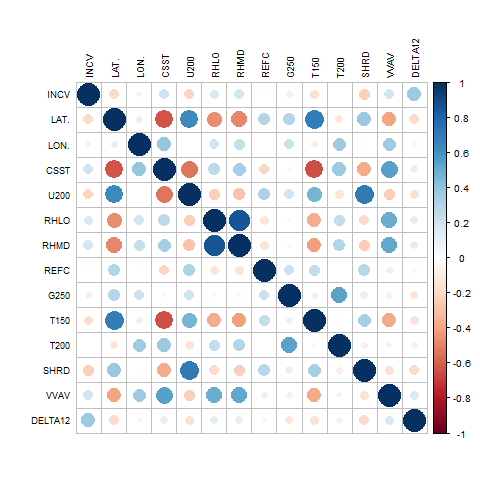
\includegraphics[width=0.5\textwidth,height=\textheight]{/home/jason/git/bda-hurricane-modeling/images/corrplot_delta_small.png}
\caption{Correlation plot of the variables we will include in the
models.}
\end{figure}

\hypertarget{prior-work-with-the-data}{%
\subsubsection{Prior work with the
data}\label{prior-work-with-the-data}}

Although the data is publicly available with no restrictions, not much
work using it can be found. This may be because of the lack of general
interest in meteorology or possibly the poor state of the documentation.
The authors of this report are not aware of any other work with this
data apart from scientific publications by the American researchers
involved in the SHIPS model development. The bulk of this research is
available at the SHIPS website:
\href{http://rammb.cira.colostate.edu/research/tropical_cyclones/ships/references.asp}{SHIPS
Model References}.

\hypertarget{brief-explanation-of-chosen-variables}{%
\subsubsection{Brief explanation of chosen
variables}\label{brief-explanation-of-chosen-variables}}

\begin{itemize}
\tightlist
\item
  \textbf{INCV}: intensity change from last time period to current time
\item
  \textbf{LAT/LON}: latitude/longitude coordinates
\item
  \textbf{CSST}: (climatological) sea surface temperature
\item
  \textbf{U200}: longitudal component of jet winds at 200 mb height
\item
  \textbf{RHLO}: relative humidity at low altitude (\textasciitilde850
  mb)
\item
  \textbf{RHMD}: relative humidity at medium altitude
  (\textasciitilde500 mb)
\item
  \textbf{REFC}: rotational eddy flux convergence (don't ask)
\item
  \textbf{G250}: temperature gradient caused by the storm, at 250 mb
\item
  \textbf{T150}: air temperature at 150 mb
\item
  \textbf{T200}: air temperature at 200 mb
\item
  \textbf{SHRD}: wind shear between 850 mb and 200 mb heights
\item
  \textbf{VVAV}: the vertical wind near sea surface (convection)
\item
  \textbf{VMPI}: a variable from Potential Intensity theory;
  theoretically representing the maximum physically possible wind
  intensity that the storm could achieve in ideal conditions
\end{itemize}

\newpage

\hypertarget{modelling}{%
\section{Modelling}\label{modelling}}

In this project we studied three different model structures with
different variable selections. Drawing inspiration from the US
government SHIPS model, all of our models are some variation of linear
regression.

\hypertarget{description-of-the-models}{%
\subsection{Description of the models}\label{description-of-the-models}}

\hypertarget{linear-regression}{%
\subsubsection{Linear regression}\label{linear-regression}}

The first model is the simplest possible case - just a linear regression
model. The mathematical statement of the model is as follows, where we
let \(N\) denote the number of regression parameters.

\[ y_{i} \sim \mathcal{N}(\alpha + X_i \cdot\beta_{N-1}, \sigma), \ i=1,\dots,r, \]
where we let \(X_i\) denote the \(i\):th row of the data,
\(\beta_{N-1}\) is an \(N-1\)-dimensional parameter vector, and \(r\) is
the number of observations (rows) in the data. The inference is done on
the parameters \(\alpha , \beta, \sigma.\) They are given the following
(weak) prior distributions.

\[\begin{bmatrix} \alpha_0 \\ \beta_{N-1,0} \end{bmatrix} \sim \mathcal{N}(\mathbf{0}_N, 10 \cdot \mathbf{I}_N), \sigma_0 \sim \textrm{Inv-}\chi^2(\tfrac{1}{10}) .\]
The Stan code for this model is the following one:

\begin{Shaded}
\begin{Highlighting}[]
\KeywordTok{writeLines}\NormalTok{(}\KeywordTok{readLines}\NormalTok{(}\StringTok{"models/linear.stan"}\NormalTok{))}
\end{Highlighting}
\end{Shaded}

\begin{verbatim}
## 
## data {
##   int<lower=0> N;
##   int<lower=0> J;
##   vector[N] y;
##   matrix[N,J] x;
##   vector[J+1] mu; // required prior means 
##   matrix[J+1, J+1] tau; // prior covariance matrix
## }
## 
## parameters {
##   vector[J+1] theta;
##   real < lower =0 > sigma;
## }
## 
## model {
##   theta ~ multi_normal(mu, tau);
##   sigma ~ inv_chi_square(0.1);
##   y  ~ normal( theta[1] + x*theta[2:J+1], sigma);
## }
## 
## generated quantities {
##   vector[N] log_lik;
##   for (n in 1:N) {
##     log_lik[n] = normal_lpdf(y[n] | theta[1] + x[n]*theta[2:J+1], sigma);
## }}
\end{verbatim}

We run this model with 4 chains for 4000 iterations using 2000 as
warm-up. We used the datasets ``A'', ``B'', and ``C'', and for all of
them, the ESS is always higher than 100, and the \(\hat{R}\) values
approximated to 1.0 for each parameter, which means that we run enough
iterations to reach convergence. If this was not the case and the
\(\hat{R}\) ratios were higher than 1, the chains would not be sampling
from the same part of the parameter space and we would need either to
increase the number of iterations or to edit the proposal distribution.
The definition of \(\hat{R}\) that we used can be found
\href{https://arxiv.org/abs/1903.08008}{here}.

\hypertarget{skew-regression}{%
\subsubsection{Skew-regression}\label{skew-regression}}

The second model is a variation of the first, where instead of a normal
distribution around the regression line, a skew-normal distribution is
used. This probability distribution has different properties, making
computation a bit less efficient, but there are scientific reasons to
believe that a skew towards higher intensity changes would be a better
fit. The model is summarized in mathematical language as follows.

\[ y_{i} \sim \textrm{SkewNormal}(\alpha + X_i \cdot\beta_{N-1}, \sigma, \psi), \ \ i=1,\dots,r, \]
where we use the same conventions as in the linear model. The priors of
the parameters are given below.
\[\begin{bmatrix} \alpha_0 \\ \beta_{N-1,0} \end{bmatrix} \sim \mathcal{N}(\mathbf{0}_N, 10 \cdot \mathbf{I}_N), \sigma_0 \sim \textrm{Inv-}\chi^2(\tfrac{1}{10}) , \ \psi_0 \sim \mathcal{N}(0,1) .\]
We run this model for the same number of iterations as before: 4000
using with 2000 as warm-up, the same number of chains: 4, and the same
datasets: ``A'', ``B'', and ``C''. But in this case we also increased
the maximum tree depth to 15. Convergence was also reached in all these
cases, as all \(\hat{R}\) values approximated to 1.0 and all ESS were
higher than 100.

\hypertarget{regression-with-changing-variance}{%
\subsubsection{Regression with changing
variance}\label{regression-with-changing-variance}}

This is another variation of the linear regression model. In this model
there is also a regression variance dependence on the wind intensity
\(V_{max}.\) This somewhat justified, since very extreme values of
\(V_{max}\) lead to volatile situations where the evolution of the storm
can be difficult to predict even for the best forecasting agencies.
There are also relatively few cases of high \(V_{max}\) since every
storm starts out weak, but only a few evolve to be high-category
hurricanes.

This model is declared in mathematical notation as follows:

\[ y_{i} \sim \mathcal{N}(\alpha + X_i \cdot\beta_{N-1}, \sigma + \gamma\vert V_{max,i} \vert ), \ i=1,\dots,r, \]
where, again, we use the same notation as before and let \(V_{max,i}\)
denote the \(V_{max}\)-value of the \(i\):th row. Note the absolute
value function in the variance section; this statement is used to ensure
that the variance remains positive. The parameters are given the priors
listed below.

\[\begin{bmatrix} \alpha_0 \\ \beta_{N-1,0} \end{bmatrix} \sim \mathcal{N}(\mathbf{0}_N, 10 \cdot \mathbf{I}_N), \ \sigma_0 \sim \textrm{Inv-}\chi^2(\tfrac{1}{10}), \ \gamma_0 \sim \Gamma(1,1) .\]
To execute this model we used 4 chains, 4000 iterations with half of
them as warm-up and a maximum tree depth of 15. We checked the
\(\hat{R}\) values for the three variable combinations (``A'', ``B'',
and ``C''), and all of them approximated to 1.0, so we can state that
the chains converged in the three cases. Moreover ESS is always high
enough.

\hypertarget{model-comparison}{%
\subsection{Model Comparison}\label{model-comparison}}

We assessed the models using leave-one-out cross-validation (LOO-CV) to
do further comparisons, and we used the r package \emph{loo} for using
PSIS-LOO as method to approximate the exact LOO given the posterior
samples.

The PSIS-LOO elpd for the basic linear model using data ``A'' is -1636.0
with 9 as effective number of parameters (p\_loo), looic of 3272.1 and
Monte Carlo Standard Error (MCSE) of 0.0. For data ``B'', the PSIS-LOO
elpd is -1633.6 with p\_loo = 10, looic = 3267.2 and MCSE = 0.1. For the
last dataset ``C'', the elpd\_loo is -1608.6, with p\_loo = 13.1, looic
= 3217.2 and MCSE = 0.1. All the Pareto k estimates are lower than 0.5
for the first two datasets, and there is only one value for ``C'' above
0.5, but it is lower than 0.7, as we can see in Figure. X. This means
that the three PSIS-LOO estimates can be considered to be reliable.

\begin{figure}
\centering
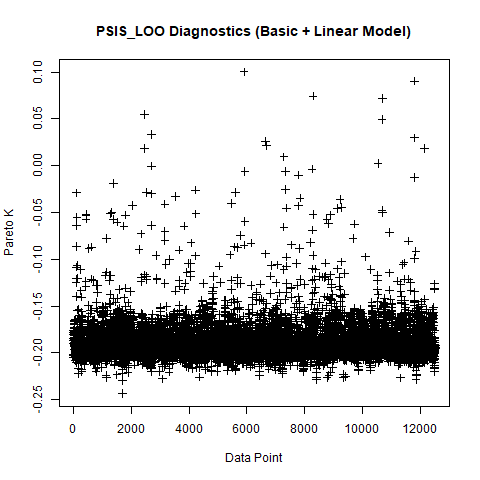
\includegraphics[width=0.7\textwidth,height=\textheight]{/home/jason/git/bda-hurricane-modeling/images/pareto_linear.png}
\caption{PSIS-LOO diagnosis for the linear model.}
\end{figure}

The model with dataset ``C'' has the highest PSIS-LOO and the lowest
looic associated to it, but in order to better assess the differences
between the datasets we have used the function \emph{loo\_compare}. This
functions computes the difference in elpd relative to the model with the
largest elpd (in this case, the ``C'' model). As we can see in Table X,
the differences in elpd and the scale relative to the standard error of
these differences indicate that the best dataset for this model
according to PSIS-LOO would be the dataset ``C''.

\begin{longtable}[]{@{}ccc@{}}
\toprule
variable set & \textbf{elpd\_diff} & \textbf{se\_diff}\tabularnewline
\midrule
\endhead
\emph{C} & 0.0 & 0.0\tabularnewline
\emph{B} & -25.0 & 6.5\tabularnewline
\emph{A} & -27.4 & 6.3\tabularnewline
\bottomrule
\end{longtable}

The PSIS-LOO elpd for the skewed-regression model using data ``A'' is
-1608.1 with p\_loo = 9.6, looic = 3272.1, and MCSE = 0.1. For dataset
``B'', the PSIS-LOO elpd is -1602.5 with p\_loo = 10.4, looic = 3205.1
and MCSE = 0.1. For the last dataset ``C'', the elpd\_loo is -1579.4,
with p\_loo = 13.3, looic = 3158.7 and MCSE = 0.1. All the Pareto k
estimates are lower than 0.5 for the first two datasets, and there is
only one value for ``C'' above 0.5, but it is lower than 0.7, as we can
see in Figure. X. This means that the three PSIS-LOO estimates can be
considered to be reliable.

\begin{figure}
\centering
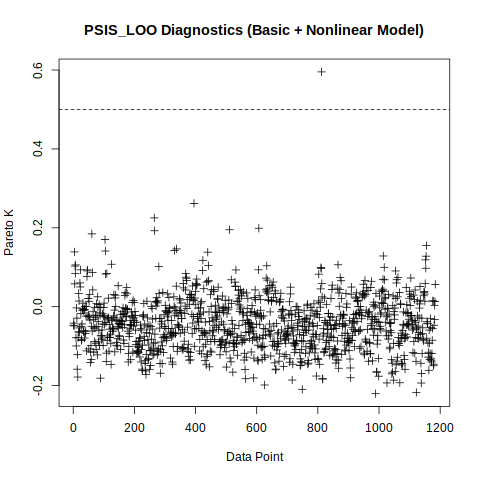
\includegraphics[width=0.7\textwidth,height=\textheight]{/home/jason/git/bda-hurricane-modeling/images/pareto_skew.png}
\caption{PSIS-LOO diagnosis for the skewed model.}
\end{figure}

\newpage

Using \emph{loo\_compare} we can observe that the best dataset for this
model would be again dataset ``C'' (Table X).

\begin{longtable}[]{@{}ccc@{}}
\toprule
variable set & \textbf{elpd\_diff} & \textbf{se\_diff}\tabularnewline
\midrule
\endhead
\emph{C} & 0.0 & 0.0\tabularnewline
\emph{B} & -23.2 & 6.2\tabularnewline
\emph{A} & -28.7 & 6.2\tabularnewline
\bottomrule
\end{longtable}

The PSIS-LOO elpd for the regression with changing variance using data
``A'' is -1440.2 with p\_loo = 7.3, looic = 2880.5, and MCSE = 0.1. For
dataset ``B'', the PSIS-LOO elpd is -1435.8 with p\_loo = 8.3, looic =
2871.5 and MCSE approximated to 0.0. For the last dataset ``C'', the
elpd\_loo is -1403.1, with p\_loo = 12.0, looic = 2806.2 and MCSE = 0.0.
All the Pareto k estimates are lower than 0.5, as we can see in Figure.
X, which means that the three PSIS-LOO estimates can be considered to be
reliable.

\begin{figure}
\centering
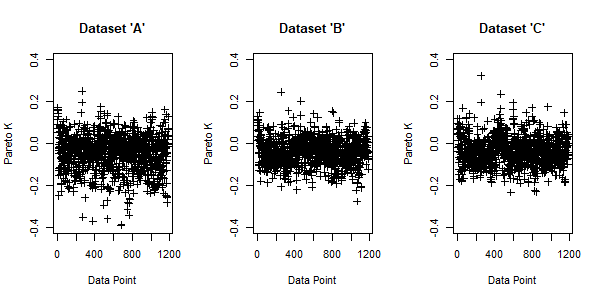
\includegraphics[width=0.7\textwidth,height=\textheight]{/home/jason/git/bda-hurricane-modeling/images/pareto_variance.png}
\caption{PSIS-LOO diagnosis for the variance model.}
\end{figure}

Using again the function \emph{loo\_compare} we can see that the best
dataset for this model would be again dataset ``C'' (Table X).

\begin{longtable}[]{@{}ccc@{}}
\toprule
variable set & \textbf{elpd\_diff} & \textbf{se\_diff}\tabularnewline
\midrule
\endhead
\emph{C} & 0.0 & 0.0\tabularnewline
\emph{B} & -32.6 & 8.2\tabularnewline
\emph{A} & -37.1 & 8.2\tabularnewline
\bottomrule
\end{longtable}

We have seen that the best dataset for all of our Stan models is dataset
``C''. If we compare now the three models using this dataset, we can see
that the best performing model according to PSIS-LOO would be the last
studied model, the regression with changing variance.

\begin{longtable}[]{@{}ccc@{}}
\toprule
Model & \textbf{elpd\_diff} & \textbf{se\_diff}\tabularnewline
\midrule
\endhead
\textbf{Variance} & 0.0 & 0.0\tabularnewline
\textbf{Skew} & -176.3 & 27.8\tabularnewline
\textbf{Linear} & -205.5 & 34.9\tabularnewline
\bottomrule
\end{longtable}

\newpage

\hypertarget{evaluation-and-potential-improvements}{%
\section{Evaluation and potential
improvements}\label{evaluation-and-potential-improvements}}

The best model - the variance regression model - was used to generate
forecasts for Hurricane Dorian - an especially powerful Hurricane that
hit the Bahamas in 2019. See the image below for a comparison between
the model predictions and Dorian's empirical intensity development.

\begin{figure}
\centering
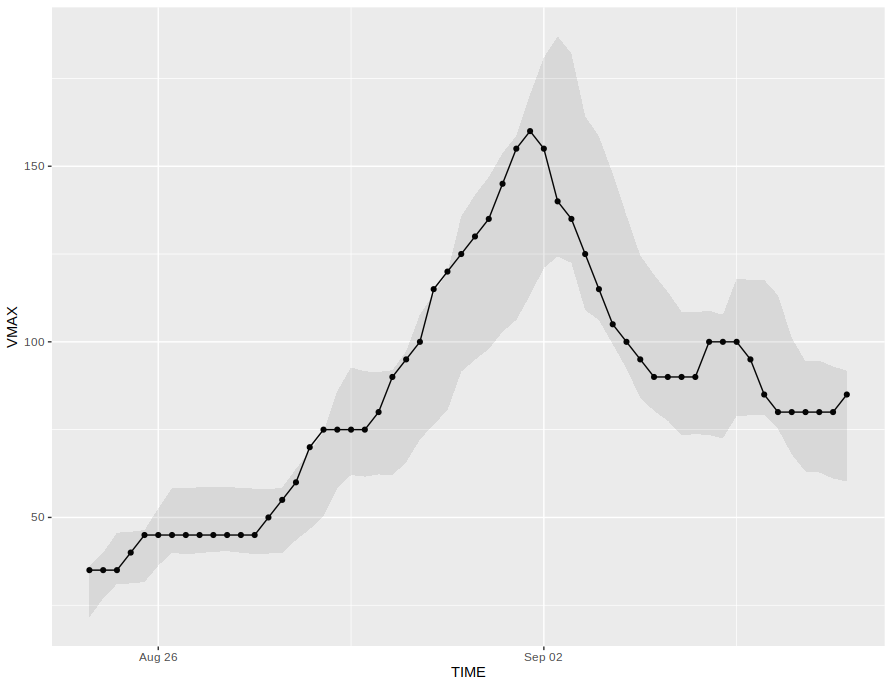
\includegraphics[width=0.75\textwidth,height=\textheight]{/home/jason/git/bda-hurricane-modeling/images/proto_eval_dorian.png}
\caption{Comparison between the true wind intensity of Hurricane Dorian
and the 12-hour forecasts from the variance model. The black line
represents the true wind intensity, while the shaded area is an 80\%
prediction interval from the model. Hurricane Dorian struck the Bahamas
as a category 5 tropical cyclone in September 2019.}
\end{figure}

Hurricane Dorian is in fact a rather exceptional storm in the sense that
it underwent a phenomenon known as \emph{rapid intensification}, which
is very difficult to predict for currently operational Hurricane models.
In particular the statistical models, including SHIPS, often fails to
predict rapid intensification, while dynamical models more often
correctly call the phenomenon (although they have worse performance in
other respects).

The Variance model developed in this project was only developed for a
12-hour forecast, but still the predicted 80\% interval contains the
true wind intensity in all time steps but one. A model based on Bayesian
computations can provide probabilistic information that is not produced
by the point estimates generated by SHIPS models, but an efficient
implementation may require a different model declaration.

There is also a variation of the SHIPS model that combines statistical
estimation of parameters with a dynamical component - the Logistic
Growth Equation Model (LGEM). A suitable next step in research could be
to implement a variation of the LGEM model in Stan and thus achieve a
probabilistic dynamical model.

Another improvement idea would be to include a time series component in
the regression models used in this report. In fact, the operational
SHIPS model contains some autoregressive parameters. The SHIPS model
used by the NHC (National Hurricane Center) also contains regression
parameters for outputs from numerical weather simulation
(i.e.~dynamical) models used by the NHC. If an agency that has access to
such model outputs were to include those parameters with the models
presented in this report, it could improve prediction intervals
significantly.

\newpage

\hypertarget{conclusions-and-discussion}{%
\section{Conclusions and discussion}\label{conclusions-and-discussion}}

Hurricane intensity forecasting is an interesting problem which still
includes unsolved scientific challenges. We have demonstrated that the
existing SHIPS architecture could potentially be improved with some
simple changes to the linear regression design and that probabilistic
information created by Stan can provide useful information. Despite
this, computational challenges may emerge if larger observation sets or
variable selections are taken. The comparative efficiency of computing a
simple regression point estimate is probably one of the reasons that the
SHIPS model is so useful.

Nevertheless, the SHIPS model is famously poor at predicting rapid
intensification - a phenomenon which remains a challenge for forecasters
despite other improvements to forecasting techniques. The best model
chosen in this report is a model which increases variance as intensity
increases, which is an imperfect way of accounting for the higher
uncertainty (which is largely due to risk of rapid
\emph{intensification} - not \emph{weakening}).

We have learned several things about hurricane forecasting during this
project. Among others, that it is still possible to find open scientific
questions and that it is easy to get started with simple models that can
issue real forecasts that provide useful information. The probabilistic
information provided by Stan also provides an interesting improvement
over black-box statistical methods, while computational issues may
somewhat hinder model development. We conjecture that Bayesian
computation may prove useful especially in analyzing individual storms
that undergo rapid intensification, since this would entail a deep
analysis of a small dataset.

\newpage

\hypertarget{appendix}{%
\section{Appendix}\label{appendix}}

\hypertarget{stan-models}{%
\subsection{Stan models}\label{stan-models}}

\end{document}
